\section{Image Segmentation Architectures}

    Fully convolutional network (FCN) is a CNN variant which is a turning point for semantic segmentation literature \cite{long2015fully}.
    After that, many variants of CNN for segmentation has been developed.
    In this section, commonly used CNNs which are used for image segmentation starting from FCN are examined.

    \subsection{Fully Convolutional Network}

        Fully convolutional networks (FCNs) indicate that the convolutional neural networks are obtained by dismantling the fully connected layers from deep CNNs \cite{ulku2019survey}.
        FCNs are built on traditional classification networks such as VGG\cite{simonyan2014very}, AlexNet \cite{krizhevsky2012imagenet}, GoogLeNet\cite{szegedy2014going}, and ResNet\cite{he2016deep}.

        Convolutional layers are used instead of fully connected layers to produce outputs with the same size of inputs  instead of classification scores which are the outputs of CNNs.
        FCNs consist of two units encoding and decoding. Convolution and subsampling operations are performed in the encoding unit to encode the lower dimensional latent space.
        Deconvolution and upsampling are performed in the decoding unit which guarantee the obtaining the same size of output with the input.
        Because FCNs do not include fully connected layers, it is faster to inference an image if they are compared with the classical CNNs.

        Besides the including convolutional layers, skip architecture is one of the main reasons that makes FCNs faster over CNNs.
        Skip architectures help to prevent losing some information which can be lost because of the dropout or any other architectural decisions which may cause losing information.
        They provide flowing the summed or concatenated data between downsampling and upsamling blocks.
        Skip connections are also preserve the localised information which may lose on pooling layers with bypassing them.

    \subsection{SegNet}

        \citet{badrinarayanan2017segnet} proposed a FCN based network architecture, called SegNet, aiming to increase the accuracy of segmentation tasks.
        As it can be seen in Figure~\ref{figure:segnet-architecture}, the encoder network of the proposed method is consist of 13 convolutional layers of VGG16 network instead of the original fully connected layers of FCN.
        A pixel-wise classification layer is added to helps the upsampling on the lower resolution images in the decoder network.
        The upsampling part is the novel improvement of SegNet.

        \begin{figure}
    \centerline{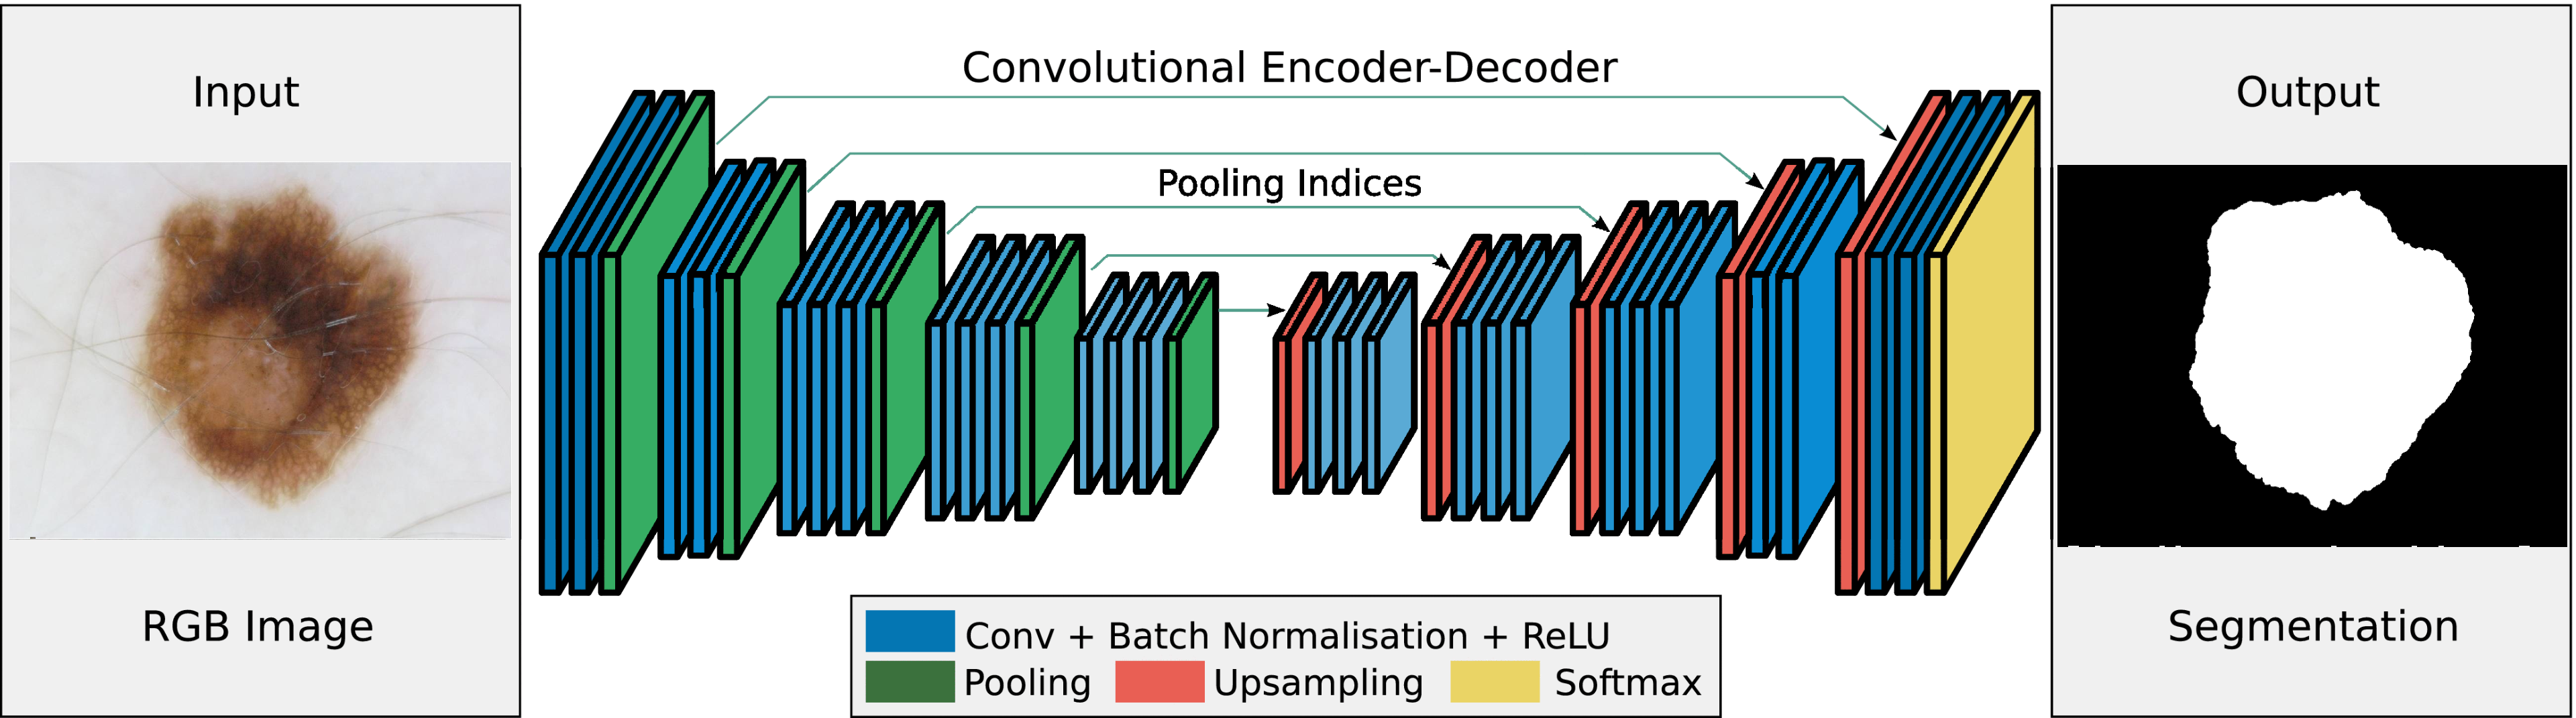
\includegraphics[width=1\columnwidth]{02-related-works/figures/segnet-architecture.png}}
    \caption{ SegNet architecture \cite{badrinarayanan2017segnet} }
    \label{figure:segnet-architecture}
\end{figure}

        Encoder is not fully connected in Segnet causes the train parameters to decrease by ~90\%.
        There is a corresponding decoder for every 13 encoders and they are responsible for upsampling of the feature map.

    \subsection{U-Net}\label{section:unet}

        \citet{ronneberger2015u} proposed a new CNN namely U-Net designed for medical imaging.
        Because medical image segmentation suffers from lack of large dataset, it is relatively hard to capture image context with localized lesions.
        U-Net aims to achieve competitive results even if the training data are relatively small.

        \begin{figure}
    \centerline{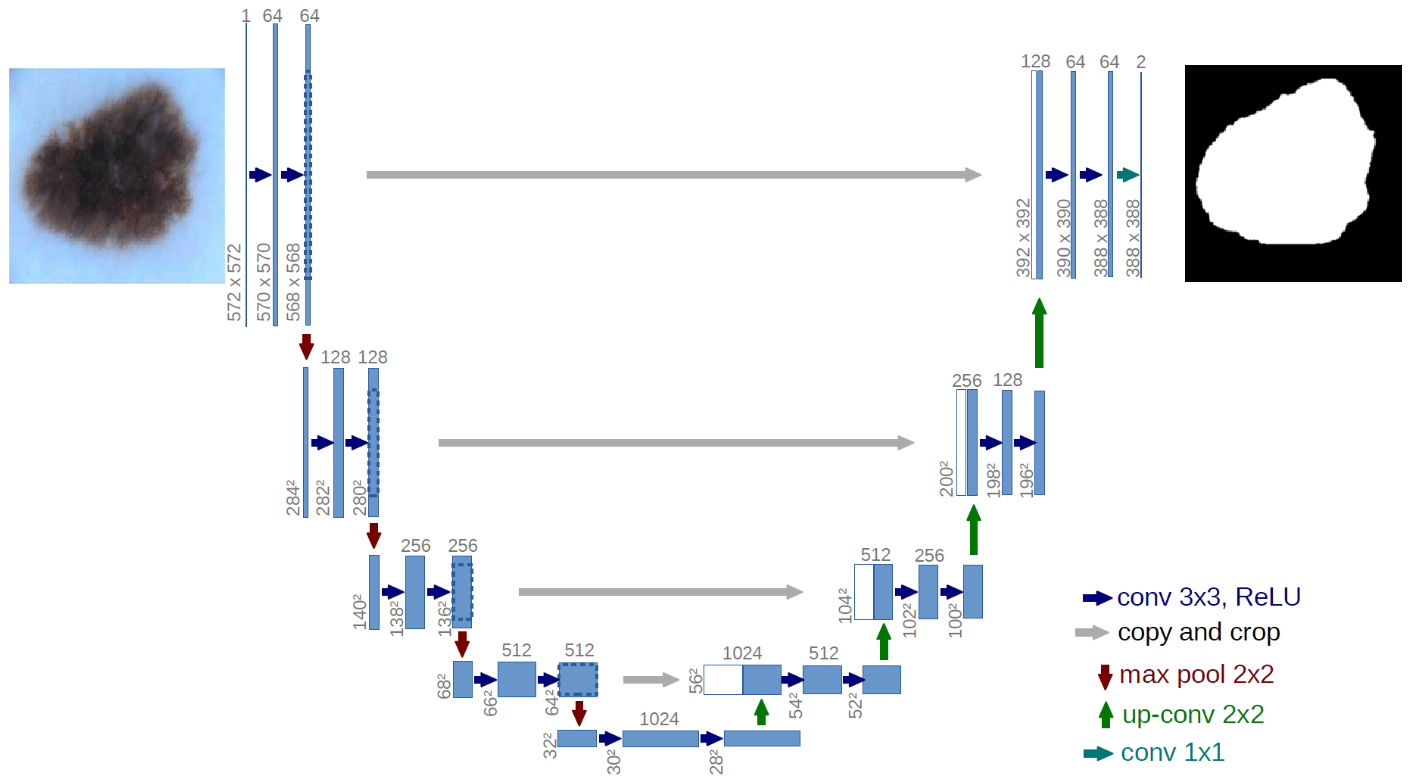
\includegraphics[width=1\columnwidth]{02-related-works/figures/u-net-architecture.png}}
    \caption{ U-Net architecture \cite{ronneberger2015u} }
    \label{fig:unet-architecture}
\end{figure}

        Classical feed-forward CNNs can learn many small information with details with the help of the fully connected layers because large datasets provide a number of parameters to train.
        On the contrary, large datasets oftenly are not exist or not accesible in medical imaging.
        Thus, if the neural network aims to accurate results with them, each image in dataset needs to be learnt deeply to extract the features.
        Up convolutions of the decoder unit which is a replacement of fully connected layers still have trainable parameters and this makes U-Net relatively more successful with smaller datasets by capturing context in detail.
        As it can be shown in Figure~\ref{figure:unet-architecture}, U-Nets are made up of contracting and expansive paths on the left and right respectively.

        The purpose of the contracting path is to increase resolutions and learn features  to capture context while the role of the expanding path is to aid in precise localization with a series of upsampling operations.
        The contracting path consist of two three-by-three convolutions followed by a ReLU and two-by-two max pooling layers.
        On the other side, up convolution layers exist to upsample the outputs.
        Skip connections help to prevent to lose the spatial context combining with upsampled outputs by transfering the low resolution features to expanding path.
        The authors used a large-weighted loss function to separate boundaries of background labels and touching segments which is a known problem of medical image segmentation.

    \subsection{Generative Adversarial Network}

        \citet{goodfellow2014generative} proposed a deep learning framework which is called generative adversarial network (GAN) consisting of two neural networks namely generator and discriminator.
        The proposed network can be considered as an autoencoder trying to produce a fake version of the real data.

        The generator which is the first part of the GANs, generates a sample and the discriminator interprets the sample as a real or fake.
        The ‘real’ means that whether the source of the data is training set. The flow can be seen in Figure~\ref{figure:gan-architecture}.

        \begin{figure}
    \centerline{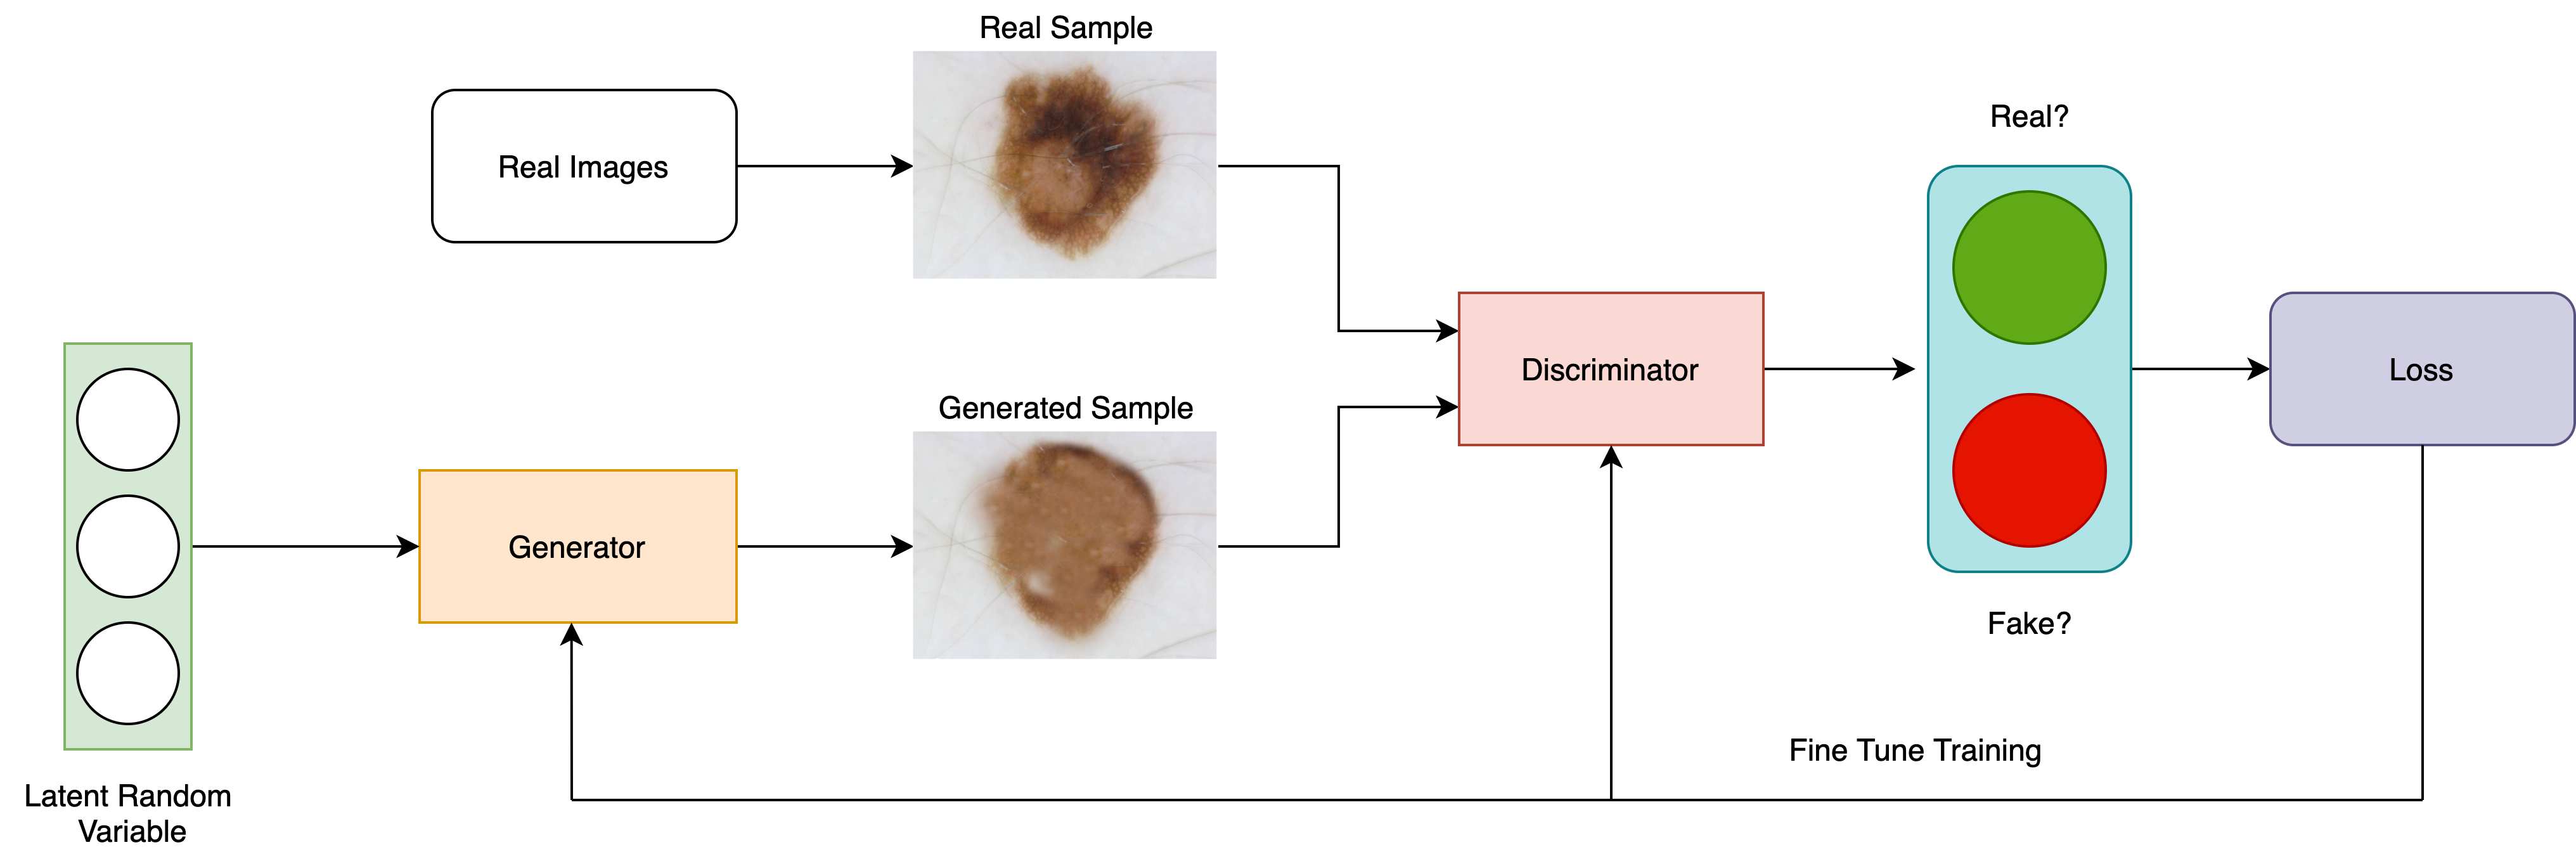
\includegraphics[width=1\columnwidth]{02-related-works/figures/gan-architecture.png}}
    \caption{ GAN architecture }
    \label{figure:gan-architecture}
\end{figure}

        It looks like a game where the generator tries to fool the discriminator with the samples it creates.
        The generator are update itself using the output of the discriminator on each iteration and gives better results.
        GANs have proved its success in many image analysis tasks, such as creating very realistic synthetic images \cite{shrivastava2017learning},
        domain adaption \cite{bousmalis2017unsupervised} and data completion \cite{yeh2017semantic}.
        Such successful applications of GANs to image processing tasks.
